\documentclass[a4paper]{article}
\usepackage[swedish]{babel}
\usepackage[utf8]{inputenc}
\usepackage[T1]{fontenc}
\usepackage{algpseudocode}
\usepackage{algorithm}
\usepackage{lmodern}
\usepackage{amsmath}
\usepackage{graphicx}
\DeclareGraphicsExtensions{.png}

\title{The Lost Vaults: Uneasy Alliance\\\small{Operativsystem och multicoreprogrammering (1DT089) våren 2013}\\\small{Slutrapport för grupp 4}}

\author{Felix Färjsjö\\(19911225-4678) \and Jimmy Holm\\(19870928-0138) \and Fredrik Larsson\\(19890422-0590) \and Anna Nilsson\\(19910804-0628) \and Philip Åkerfeldt\\(19920508-1335)}

\date{\today\\Version 1.0}

%Döp om pseudokod.
\floatname{algorithm}{Algoritm}
\renewcommand{\algorithmicindent}{8 pt}
\begin{document}
\maketitle
\thispagestyle{empty}
\newpage
\setcounter{page}{1}
\pagenumbering{Roman}

\tableofcontents
\listoffigures
\newpage
\setcounter{page}{1}
\pagenumbering{arabic}
\section{Inledning}
Att spela spel över internet är en del av vår kultur som antagligen aldrig kommer försvinna. Det är ett sätt att umgås och samarbeta, ofta med människor man aldrig har mött. 
På många platser i världen är gigantiska servrar igång dygnet runt för att hantera förfrågningar från miljontals användare, och tusentals programmerare gör sitt bästa för 
att ge människor en så bra användarupplevelse som möjligt. 
För att detta ska vara möjligt krävs mycket av serverprogrammen. 
Servrarna ska kunna hantera många förfrågningar med låg fördröjning, samtidigt som de måste koordinera händelser så att det som en användare gör också ska påverka dem i anslutning till den. 
Serverprogrammen ska också gärna vara finkornigt modulariserade för att möjliggöra parallellutveklingen av serverprogrammen på ett fungerande sätt.  
 
Vi kände att komplexiteten av att göra ett multiplayer onlinespel var något som utmanade och intresserade oss, då det gav upphov till intressanta problem som kunde lösas med hjälp av concurrency. 
Vi har skapat ett serverbaserat spel, som kommunicerar med användaren via en TCP/IP uppkoppling till användarens klient-program. Servern består av flera självständiga aktörer som interagerar
genom att skicka meddelanden fram och tillbaka. Detta ger oss ett bekvämt sätt att skriva fungerande spellogik, utan att behöva bry oss om att låsa delad data.

Spelet kallas \textit{The Lost Vaults - Uneasy Alliance} och är ett semi-traditionellt MUD där användaren interagerar med andra spelare och tar del i uppdrag. 
Detta sker i grupper av flertal spelare som tillsammans arbetar mot ett gemensamt mål samtidigt som varje enskild gruppmedlem har en personlig agenda som endast 
gagnar den enskilda invididen. Möjligheten finns att utforska som enskild individ, men fokuset för spelet ligger i den dynamik som följer av 
interaktionen med andra spelare. Spelet utspelas på två olika platser, i City och i Dungeon; där City är staden där spelarna samlas efter tidigare utforskningar, 
kan fylla på förnödenheter samt forma grupper för att gå ner i Dungeons. Dungeons är en procedurellt genererad uppsättning rum fyllt med monster, fällor och skatter. 
Varje grupp spelare får alltså sin egen unikt genererade Dungeon när gruppen går ner i dessa magiska grottor under staden. Väl inne ges 
gruppen en eller flera uppdrag som bör fullbordas innan de kommer upp till ytan igen.

Relationen mellan konceptet concurrency och vårt projekt är förmågan att ha fler än en spelare aktiva i spelet samtidigt och se hur dessa interagerar med varandra, samt flertalet 
aktiva spelområden körandes samtidigt och oberoende av varandra.

\section{Systemarkitektur}
\subsection{Design}
Systemarkitekturen som beskrivs i detta dokument är uppdelat i två delar vilka beskriver akritekturen för klienten samt servern. Med tanke på att både klienten och servern är skrivna i Scala och körs via Java Virtual Maschine både servern och klienten kan köras på alla plattformar som stödjer Java VM 1.7.
\begin{figure}[hbt]
\centering
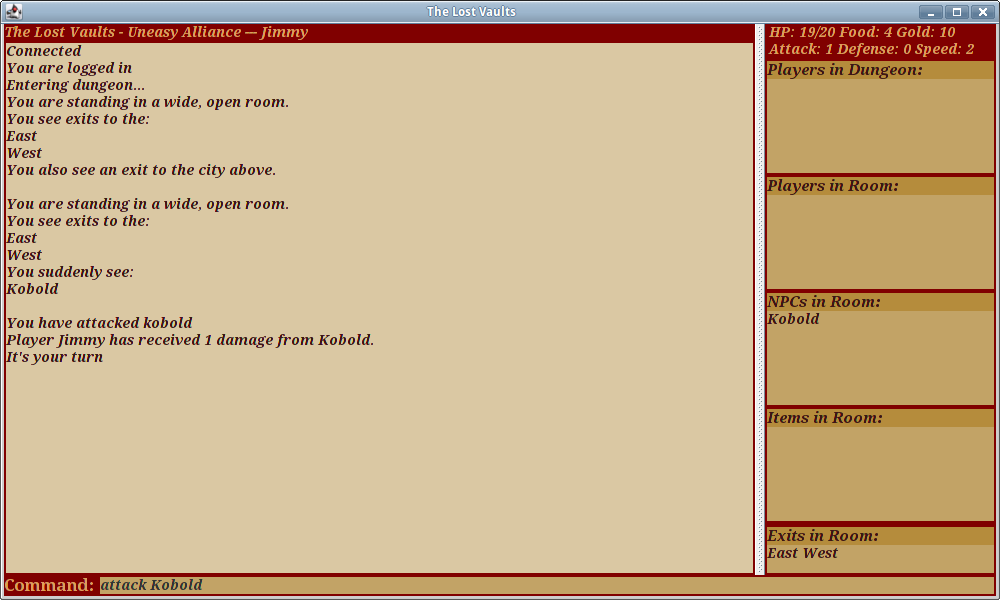
\includegraphics[width=1.0\textwidth]{client}
\caption{\label{fig:Client}Klientens användargränssnitt.}
\end{figure}

\subsection{Klient}
Designen för klienten till Lost Vaults är utvecklad för att efterlikna en indirekt terminal, där ingen logik används förutom att skicka förfrågningar och 
ta emot samt tolka svaren på förfrågningar. Konceptet för en indirekt terminal valdes för att kunna åstadkomma en implementation hos klienten som lätt kan utökas när serverns implementation av spelets logik ökar. Detta betyder med andra ord ett system som kan utkökas enkelt endast genom att addera nya förfrågningar och svar.

Som Figur 1 illustrerar är klientfönstret uppdelat i flera textfält som visar relevant information för spelaren. Huvudområdet är för vanliga server-svar och kommer innehålla beskrivningar 
av rummet, meddelanden i spelarchatten, meddelanden med systeminformation och liknande. Klientens högra sida är reserverat för ständig information som spelaren behöver ta del av snabbt. 
Den övre delen innehåller information om spelarens egen karaktär, där spelarens liv och stridsegenskaper samt hur mycket mat gruppen har listas. 

Den nedre delen av fönstret innehåller kommandoraden, där spelaren skriver in kommandon i enlighet med ett strikt syntax. När klienten startas välkomnas spelaren 
av ett centrerat fönster för inloggning. Här kan spelaren skriva in sitt användarnamn och lösenord samt IP:n tillhörande den server som spelaren vill koppla upp sig mot. 

Klientens GUI är implementerat i Javas Swing UI bibliotek och integrerat i Scala för att använda Akkas TCP funktionalitet.

\begin{figure}[hbt]
\centering
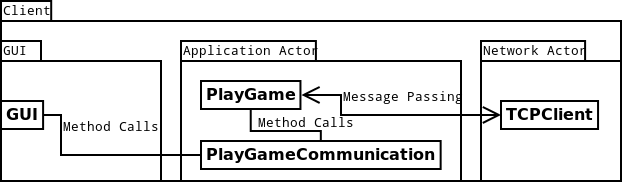
\includegraphics[width=1.0\textwidth]{clientuml1}
\caption{\label{fig:ClientArch}Klientens klassmodell.}
\end{figure}
    
\subsubsection{Klassmodell}
Klienten är strukturerad i fyra distinkta klasser som beskrivs i Figur \ref{fig:ClientArch}. Klasserna PlayGame och PlayGameCommunication arbetar 
tillsammans för att skapa en brygga mellan TCP lagret och GUI:t, där PlayGame accepterar meddelanden från TCPClient och skickar dem 
vidare till GUI via PlayGameCommunication. Samtidigt så skickas data från GUI över nätverket via metodanrop i PlayGameCommuncation till 
PlayGame för att sedan hamna hos TCPClient.

\subsection{Server}
Systemarkitekturens serverdel är uppdelad i sektionerna Aktörmodell och Klassmodell. Den första delen beskriver funktionen hos de olika aktörlagren i Lost Vaults servern och 
den andra ger en  beskrivning av serverns klassförhållanden.

\begin{figure}[hbt]
\centering
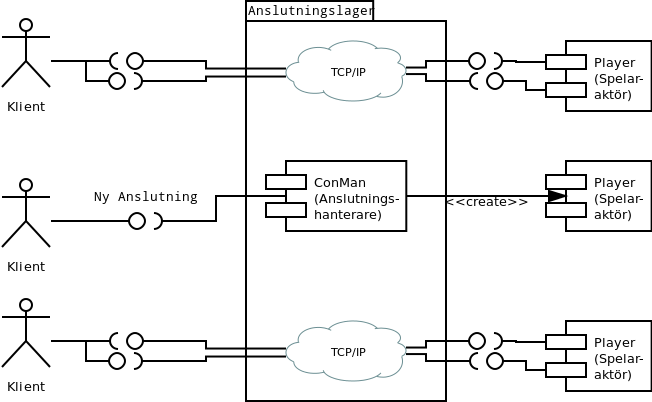
\includegraphics[width=1.0\textwidth]{serverActorModel2-1}
\caption{\label{fig:ConManPlayer}Figur över förhållandet mellan ConMan och Player.}
\end{figure}
\subsection{Server-side}

\subsubsection{Aktörmodell}
Serverdelen är uppdelad i flera processer via Akkas aktörbibliotek för att upprätthålla Actor Concurrency-modellen i enlighet med Figur \ref{fig:ConManPlayer} och Figur \ref{fig:ServerActorModel}. 
Endast två typer av aktörer kommmunicerar direkt med nätverket via TCP/IP, ConManaktören och Playeraktörerna. ConManaktören har som syfte att hantera inkommande anslutningar samt ansvarar 
för att skapa Playeraktörer som nya högnivå aktörer innan de registreras som den nyetablerade anslutningens lyssnare. Som lyssnare kommer Playeraktören ta emot och skicka data 
över nätverket. Playeraktören styr över alla attribut relaterade till sin klient, som exempelvis spelarens attribut och för att verifiera 
inloggningsförsök via kommunikation med PlayerMap och en databas innehållande inloggningsinformation. Det är även via Playeraktören andra aktörer kan skicka meddelanden över nätverket vid behov. 

PlayerMapaktören och GroupMapaktören fyller två specifika och snarlika funktioner. PlayerMap mappar en sträng, namnet på en uppkopplad spelare, till den aktör som kontrollerar 
spelaren med det eftersökta namnet. Genom denna aktör kan en annan aktör snabbt och enkelt skicka meddelanden till en specifik spelare baserat på dess namn - 
ett viktigt kommando som agerar på följande sätt är exempelvis “WHISPER”. PlayerMap möjliggör även ett snabbt och enkelt sätt för Playeraktören att försäkra 
sig om att det inte existerar flera spelare med samma namn på servern.

\begin{figure}[hbt]
\centering
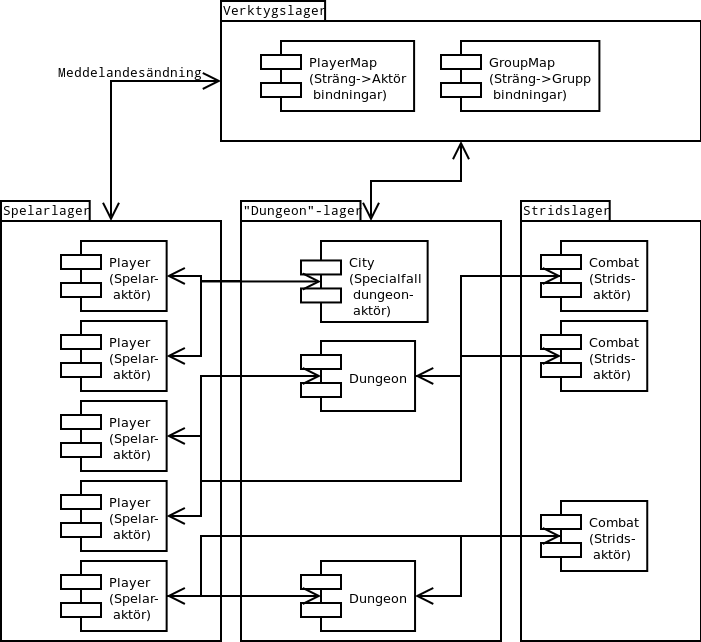
\includegraphics[width=1.0\textwidth]{serverActorModel2-2}
\caption{\label{fig:ServerActorModel}Modell över de olika aktörernas sammanhang.}
\end{figure}

GroupMapaktören fyller en liknande funktion som PlayerMap, men länkar istället namnen på spelarna med spelargrupper istället för spelaraktörer. 
En spelargrupp är en samling av en eller fler spelare som tillsammans kan gå ner i en Dungeon, som är procedurellt genererad för just dem. Syftet med 
denna aktör är att underlätta skapandet av spelargrupper samt anslutning till redan existerande spelargrupper. Genom att använda GroupMap räcker det att ansluta sig till en 
spelare via dess namn för att inkluderas i denna spelares grupp, eller för att skapa en ny grupp med denna spelare.

De två resterande lagren av aktörer som servern använder är Dungeonlagret och Stridslagret, och det är dessa som utför spelets logik. 
Det existerar ett speciellt tillstånd av Dungeonaktören, kallat Cityaktören. City existerar ständigt 
under serverns livstid och hanterar spelets sociala aspekt, såsom chattande och skapandet av grupper. 
Det som Dungeonaktören ansvarar för är genererandet och hanterandet av den procedurellt skapade 
grotta som består av multipla och sammanlänkade rum i ett tvådimensionellt rutnät. Det är i dessa rum som spelare kommer kunna göra uppdrag, 
finna skatter, slåss mot monster eller spelare etc. Dungeonaktören ansvarar även för koordinationen av alla spelare som finns i grottan. 
Ett exempel på detta är kommandot “SAY”  som ska skickas till relevanta spelare. 
Strider koordineras av sin egna aktör, en finit tillståndsmaskin kallad Combat, som sköter turordning av spelare och monster vid strid. Varje rum i en Dungeon kan innehålla en
referens till en Combat, vilket leder till att det som max kan vara upp till en combat aktiv per rum. Combataktören skapas då spelare går i strid mot monster eller andra spelare
och terminerar när det inte längre finns någon som anfaller någon annan.

Efter att Cityaktören har skapat en Dungeonaktör ansvarar den nya aktören för sin egen livslängd och avsutar sig själv endast när det inte längre finns några spelare i den.

\begin{figure}[hbt]
\centering
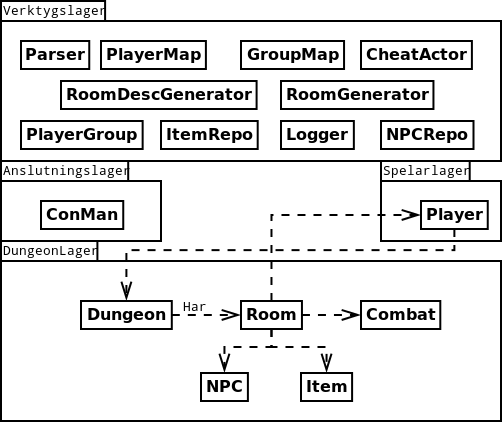
\includegraphics[width=1.0\textwidth]{serverUml2}
\caption{\label{fig:ServerKlassModell}Modell över serverns klassstruktur}
\end{figure}

\subsubsection{Klassmodell}
Figur \ref{fig:ServerKlassModell} visar de olika klasserna i serverimplementationen.
De är uppdelade i fyra lager; Verktygslagret, Anslutningslagret, Spelarlagret och Dungeonlagret. Indelningen i dessa lager följer till stor del
den indelning som gjorts i vilka klasser är sina egna aktörer. Undantagen till detta är verktygslagret, där klasserna PlayerMap, GroupMap och CheatActor är sina egna aktörer samt 
Combat klassen som i denna figur flyttats från sitt egna lager (se figur \ref{fig:ServerActorModel}) för att visa dess täta koppling med Room klassen.

Bortsett från RoomGenerator och RoomDescGenerator är alla klasser i Verktygslagret Singletons. Lagret tillhandahåller  understödjande funktionalitet till de andra klasserna.
Anslutningslagret är ingångspunkten till servern över nätverket genom Akkas TCP bibliotek. Vår anslutningshanterare, ConMan, agerar som en singleton och endast en 
instans av denna ska existera vid en given tidpunkt. ConMan är den klass som lystnar efter och godtar anslutningar från klienter, samt skapar nya Player-instanser vid nyupprättad anslutning.

Dungeonlagret innehåller de klasser som är viktiga för spelets logiska funktioner. Lagret innehåller dungeonklassen, som ansvarar över en mängd slumpmässigt genererade rum, som i sin tur
ansvarar för aktiva strider samt icke-spelarkaraktärer och objekt. Tidigare design visar att Item klassen används som superklass till olika typer av objekt. Vi valde dock att platta till 
vår klasshierarki och förenkla designen genom att låta alla typer av objekt vara instanser av Item klassen med olika attribut. På samma sätt valde vi att göra oss av med distinktionen mellan
goda och onda icke-spelarkaraktärer, och har istället valt att implementera enbart monster.

\section{Utvecklingsverktyg}

I detta projekt användes flera olika verktyg för att underlätta utvecklingen. Då vi använt Scala som vårt val av programspråk skrevs i princip all vår kod i Eclipse. 
Detta då vi anser att det i särklass är det enklaste sättet att utveckla kod till Java eller Scala. Även fast all kod är skriven i Eclipse använder vi Ant Build System 
för automatiserad kompilering samt vid byggandet av vår klient och server; som efter kompilering är klar att köras i Java Virtual Machine. 

För hanteringen av versionskontroll har vi använt det tillförlitliga och välkända verktyget Git. Vi satte upp ett nytt git repository på Github.com specifikt för detta 
projekt och valet av Git gjordes på grund av dess styrkor samt att vi är vana användare av det.

Testandet av vår kod görs med ScalaTest ramverket samt ett Ant Build skript som ger oss möjligheten till automatiskt byggande och körning av tester.

Sammansättningen av dokumentationen utförs med Scaladoc på grund av dess likhet med JavaDoc, ett verktyg vi är vana med att använda, och Ant har reviderats för att automatiskt 
bygga dokumentationen.

\section{Implementation}

\subsection{Programspråk}
För att möjliggöra massiv concurrency med många individuella aktörer har vi gjort vårt projekt i Scala. Scala är bra för skalbarhet, vilket innebär att vårt program kommer fungera bra oavsätt om det är tio användare online eller om det är tio tusen. En annan anledning till att vi valde Scala är att Scala är ett objektorienterat språk, vilket passade nära med det tänket vi hade när vi skapade programmet. Vi fokuserade på att skapa objekt som interagereade på rätt sätt med varandra, snarare än att skriva kod som ska exekveras i en särskild ordning.

Scala bygger på Java, och erbjuder därför liknande syntax. Detta innebar att övergången mellan att skriva Java och Scala var en någorlunda mjuk sådan, koden var ganska lättigenkännlig samtidigt som vi fick fördelarna med att kunna utveckla skalbart. Några nackdelar med Scala som vi finner nämnvärda är exempelvis att det, trots likheter med Java, tog en viss tid att sätta sig in i det nya 
språket vilket kan ha motarbetat utvecklingen gämfört med om vi hade valt ett annat språk som vi var mer bekanta med.

Genom rekommendationer av skaparna bakom Scala och via språkets styrkor och enkelhet, beslöt vi oss för 
att använda Akka som vårt aktörbibliotek. Detta för att kunna använda Akkas TCP-bibliotek för nätverkskommunikationen. Bibliotekets enkla integration var en av punkterna som ledde till vårt beslut att använda Scala och Akka som val av programspråk och aktörbibliotek.

Java var det språket vi valde att använda vid skapandet av det grafiska gränssnittet som spelaren agerar mot. Vårt val grundade sig i biblioteket Swing som Java tillhandahåller. 
Med hjälp att detta bibliotek var skapandet av det grafiska gränssnittet en relativt enkel process. Likt många andra av Javas bibliotek var dokumentationen välskriven och enkel 
att använda vilket underlättade processen. En annan aspekt som fick oss att välja Java för just denna del var att vi ville kunna kommunicera med resterande kod, skriven i Scala, 
på ett enkelt sätt och detta kunde uppnås utan problem då Scala är byggt utifrån Javas Virtuella Maskin. 

\subsection{Algoritmer}
För att spelarna alltid skall få  nya och intressanta upplevelser bestämde vi oss för att skriva en algoritm för slumpmässig generering av rum som spelarna kan utforska. Vi
bestämde oss för att nyttja ett rutnät där varje cell representerar ett rum. Spelare kan ta sig från rum till rum via utgångar placerade på några av eller alla rummens fyra väggar.
Vår algoritm skall även säkerställa att inga rum skapas som inte går att nå från ingången. Algoritm \ref{alg:RoomGen} beskriver med pseudokod den algoritm vi bestämde oss för att använda.
\begin{algorithm}
\caption{Procedurell Rumsgenerering.}
\label{alg:RoomGen}
\begin{algorithmic}[1]
\Function{generateRooms}{Bredd, Höjd}
\State  $Rooms$ = Array[Bredd * Höjd]
\State  $StartRoom$ = slumpmässig cell i $Rooms$
\State  $CreatedRooms$ = $0$
\State  $GoalRooms$ = önskat antal skapade rum
\Repeat
\State $ToConnect$ = List()
\State $NextRoom$  =  Slumpat rum $x$ ur $Rooms$ där $x.created = false$
\State $NextRoom.created$ = $true$
\State $ToConnect.Insert NextRoom$
\While{$NextRoom.connected \neq true$}
\State Välj en slumpmässig riktning, viktad mot $StartRoom$
\State $NextRoom$ = den cell i $Rooms$ som är ett steg i vald riktning
\If {$NextRoom.created = true$ och $NextRoom.connected \neq true$}
\If {Andra riktningar har inte prövats}
\State Välj ny riktning och börja om från $13$
\ElsIf{Alla riktningar har misslyckats}
\State Gå tillbaka ett rum ur $ToConnect$ och börja om från $12$
\If{Alla möjliga riktningar prövats i alla rum ur $ToConnect$}
\State Börja om från $7$
\EndIf
\EndIf
\ElsIf{$NextRoom.created = false$}
\State Lägg $NextRoom$ först i $ToConnect$
\EndIf
\EndWhile
\While{$|ToConnect|$}
\State Anslut $NextRoom$ med $ToConnect$
\State Sätt $NextRoom.connected = true$
\State Plocka ut $head$ från $ToConnect$ och tilldela den till $NextRoom$
\State Öka $CreatedRooms$ med $1$
\EndWhile
\Until{$CreatedRooms \geq GoalRooms$}
\EndFunction
\end{algorithmic}
\end{algorithm}

\subsection{Datastrukturer}
Under projektets gång har vi använt oss av Scalas standarbibliotek för datastrukturer där vi behövt använda datasamlingar. 
Förutom arräer och listor har vi använt oss av Hashmap för att kunna koppla spelarnamn med aktörer och spelargrupper, vilket ses i klasserna
PlayerMap och GroupMap.

\subsection{Concurrency}
Flera spelare samtidigt
Skicka meddelanden - jobbigt när man bara vill ta reda på ett värde - skicka meddelanden fram och tillbaka. Men ingen risk för deadlock då all kommunikation sker via meddelanden. 
Meddelanden är ej synkrona, vilket märks då en spelare ibland kan bli slagen efter att den har dött (det ser uut så i prompten eftersom meddelandena kommer så, men det är inte sant)
För att skapa en slags synkronisering har vi använt FSM, vilket kräver att man är i en särskild state för att kunna ta emot ett särskilt meddelanden. 

\section{Slutsatser}
Vårt slutresultat är ett textbaserat multiplayer dungeon spel. I spelets startrum kan man chatta med de andra spelarna som är online genom whisper (personligt meddelande) eller say (till alla spelare i rummet). Där kan man också forma en grupp så att man tillsammans med andra spelare kan gå ner i en dungeon och börja spela. Väl nere i en dungeon kan man chatta som vanligt, men man kan också plocka upp saker som man hittar i grottan, börja slåss mot en spelare eller NPC som är i rummet och man kan gå till andra rum. När detta sker uppdateras klienten på korrekt sätt, så att spelaren får information om vad som händer i grottan.
Vi har också skapat en \textit{god mode} som gör att man i terminalen kan ge spelare speciella items, samt hela den så att den får fullt hp. Detta gjorde vi för att kunna testa spelet och för att kunna visa upp hur det faktiskt fungerar utan att behöva leta genom alla rum i en dungeon.

Något vi gjorde bra var att vi gjorde klart det essentiella för huvudmålet med projektet, att uppnå concurrency på något sätt. Spelet hanterar många individuella aktörer, och klarar av att hantera massiva uppkopplingar mot dess server. 
Då den delen av projektet var klart kunde vi utöka produkten med funktioner för att göra spelet roligare och mer interaktivt. 
Implementation av föremål och monster att slåss mot i grottan. 
Något vi lärt oss är att skriva nätverkskod. Vi har även fått kunskap i ett nytt programspråk.
Det vi tycker har varit svårt var bland annat att integrationstesta våra aktörer. Svårigheterna uppstod på grund av bristande 
information att ta del av om hur vi skulle gå till väga för att göra detta. En annan sak som också varit relativt svår var att 
begränsa oss när det gällde den utsträckning för vilket spelet skulle utvecklas. Att begränsa oss till en rimlig nivå för spelet 
och samtidigt ha det tillräckligt intressant för den som spelar visade sig vara mer utmanande än vi först trott.

En stor sak som vi inte hann med under projektets gång är att implementera uppdrag. Detta är vad vårt nästa steg skulle vara, nu när det grundläggande fungerar som det ska.

\section{Appendix}

Scala 2.10.4, Akka 2.3.2, SLF4J 1.7.7, Slick 2.0.2, SQLite JDBC 3.7.2

https://github.com/senilica/LostVaults/

Vilka versioner av till exempel Erlang, Java, Python etc har använts?
Hur kan koden laddas ner? Finns koden tillgänglig på till exempel GitHub eller Bitbucket eller som Tar arkiv?  Beskriv projektets katalogstruktur.
Vilket stöd för automatiserad testning finns och hur används det, till exempel JUnit (Java), EUnint (Erlang) eller PyUnit (Python)?
%Vilket stöd för automatiserad generering av dokumentation finns och hur används det, till exempel Doxygen (C, C++, C\#, Fortran, Java, Objective\­C, PHP, Python), EDoc (Erlang), Pydoc (Python), Javadoc (Java)?
Hur kompileras systemet?
Hur startas systemet? tryck på play


\end{document}
